\[
\pm c\sqrt{\sigma_{11}+\sigma_{12}}\begin{bmatrix}\dfrac{1}{\sqrt{2}}\\[2ex]\dfrac{1}{\sqrt{2}}\end{bmatrix}
\quad\text{和}\quad
\pm c\sqrt{\sigma_{11}-\sigma_{12}}\begin{bmatrix}\dfrac{1}{\sqrt{2}}\\[2ex]-\dfrac{1}{\sqrt{2}}\end{bmatrix}
\]
\hfill$\blacksquare$

我们指出在结论 4.7 中,选择 $c^{2}=\chi_p^{2}(\alpha)$,这里 $\chi_p^{2}(\alpha)$ 是自由度为 $p$ 的 $\chi^{2}$ 分布的上 $(100\alpha)$ 百分位数,将导致含概率 $(1-\alpha)100\%$ 的轮廓线. 特别对 $p$ 维正态分布,以下命题是正确的:

\begin{mvbox}
满足
\phantomsection\label{eq:4-8}
\begin{equation}
(\mathbf{x}-\boldsymbol{\mu})'\boldsymbol{\Sigma}^{-1}(\mathbf{x}-\boldsymbol{\mu})\leqslant\chi_p^{2}(\alpha)
\tag{4-8}
\end{equation}
的 $\mathbf{x}$ 值的实心椭球有概率 $1-\alpha$.
\end{mvbox}

\hyperref[fig:4.2]{图 4.2} 中的二元正态分布的概率 $50\%$ 和 $90\%$ 的常数密度轮廓线如\hyperref[fig:4.4]{图 4.4} 所示.

\begin{mvfigure}
\begin{minipage}{0.48\linewidth}\centering
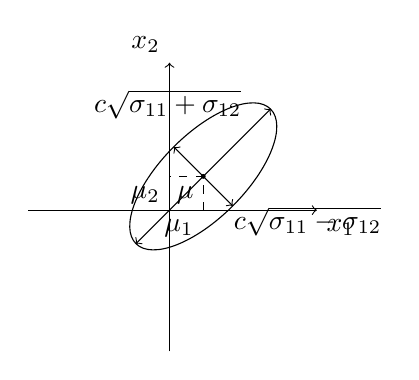
\begin{tikzpicture}[scale=0.78]
  \draw[->] (-2.3,0) -- (2.4,0) node[below right]{$x_1$};
  \draw[->] (0,-2.3) -- (0,2.4) node[above left]{$x_2$};
  \coordinate (m) at (0.55,0.55);
  \draw[dashed] (0.55,0) -- (0.55,0.55) -- (0,0.55);
  \fill (0.55,0.55) circle (0.04);
  \node[below left] at (0.55,0.55) {$\mu$};
  \node[below left] at (0.55,0) {$\mu_1$};
  \node[below left] at (0,0.55) {$\mu_2$};
  \draw[rotate around={45:(0.55,0.55)}] (0.55,0.55) ellipse (1.55 and 0.68);
  \draw[<->] (0.55-1.10,0.55-1.10) -- (0.55+1.10,0.55+1.10);
  \node[above left] at (0.55+0.78,0.55+0.78) {$c\sqrt{\sigma_{11}+\sigma_{12}}$};
  \draw[<->] (0.55-0.48,0.55+0.48) -- (0.55+0.48,0.55-0.48);
  \node[below right] at (0.55+0.34,0.55-0.34) {$c\sqrt{\sigma_{11}-\sigma_{12}}$};
\end{tikzpicture}
\phantomsection\label{fig:4.3}\mvcap{图 4.3\quad 对于 $\sigma_{11}=\sigma_{22}$ 且 $\sigma_{12}>0$(或 $\rho_{12}>0$)的\\ 二元正态分布的常数密度轮廓线}
\end{minipage}\hfill
\begin{minipage}{0.48\linewidth}\centering
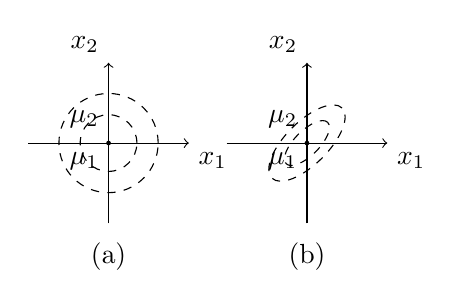
\begin{tikzpicture}[scale=0.6]
  \begin{scope}
    \draw[->] (-1.7,0) -- (1.7,0) node[below right]{$x_1$};
    \draw[->] (0,-1.7) -- (0,1.7) node[above left]{$x_2$};
    \draw[dashed] (0,0) circle (0.6);
    \draw[dashed] (0,0) circle (1.05);
    \draw[dashed] (0,-0.05) -- (0,0);
    \fill (0,0) circle (0.05);
    \node[below left] at (0,0) {$\mu_1$};
    \node[below left] at (0,0.9) {$\mu_2$};
    \node[below] at (0,-1.9) {(a)};
  \end{scope}
  \begin{scope}[xshift=4.2cm]
    \draw[->] (-1.7,0) -- (1.7,0) node[below right]{$x_1$};
    \draw[->] (0,-1.7) -- (0,1.7) node[above left]{$x_2$};
    \draw[dashed,rotate around={45:(0,0)}] (0,0) ellipse (1.05 and 0.45);
    \draw[dashed,rotate around={45:(0,0)}] (0,0) ellipse (0.62 and 0.26);
    \fill (0,0) circle (0.05);
    \node[below left] at (0,0) {$\mu_1$};
    \node[below left] at (0,0.9) {$\mu_2$};
    \node[below] at (0,-1.9) {(b)};
  \end{scope}
\end{tikzpicture}
\phantomsection\label{fig:4.4}\mvcap{图 4.4\quad \hyperref[fig:4.2]{图 4.2} 中的二元正态分布的概率 $50\%$ 和\\ $90\%$ 的常数密度轮廓线}
\end{minipage}
\end{mvfigure}

当\hyperref[eq:4-3]{式(4-3)}中的距离平方是零——即当 $\mathbf{x}=\boldsymbol{\mu}$ 时,\hyperref[eq:4-4]{式(4-4)}中的 $p$ 元正态密度有最大值. 因此,$\boldsymbol{\mu}$ 是密度最大的点,或众数,也是 $\mathbf{X}$ 的期望值(或均值). $\boldsymbol{\mu}$ 为多元正态分布的均值,这是由常数密度轮廓线所显示的对称性得出的:这些轮廓线中心在 $\boldsymbol{\mu}$ 或对称于 $\boldsymbol{\mu}$.

\mvsub{多元正态分布的可加性}

在我们对于统计模型和方法的解释中,必须重复正态分布的一些性质. 这些性质使我们有可能轻松熟练地使用正态分布,并且正如我们在 4.1 节所指出的,这些性质对正态分布的广泛运用起到了一部分作用. 我们可以相当简洁地陈述主要性质,并很快从数学角度详细讨论.

对于具有多元正态分布的随机向量 $\mathbf{X}$,下列性质是正确的:

1. $\mathbf{X}$ 的分量的线性组合是正态分布.

2. $\mathbf{X}$ 的分量的所有的子集有一个(多元)正态分布.

3. 零协方差意味着相应的分量是独立分布的.

4. 分量的条件分布是(多元)正态的.

这些性质在下面的结论中用数学方法重新表述. 这些结论中的多数用例题来说明. 所给出的证明有助于提高对矩阵运算的理解,并且促进对这些结论相继建立的方式的认识.

结论 4.2 可以用来作为正态分布的一个实用的定义. 采用该定义,以后的性质几乎可以直接得到. 结论 4.2 的部分的证明指出,一个正态密度的线性组合定义如何与\hyperref[eq:4-4]{式(4-4)}中的多元密度相联系.

\mvthm{结论 4.2}{若 $\mathbf{X}$ 的分布为 $N_p(\boldsymbol{\mu},\boldsymbol{\Sigma})$,则多个变量的任何线性组合 $\mathbf{a}'\mathbf{X}=a_1X_1+a_2X_2+\cdots+$}
